\chapter{Background Knowledge}

\section{A brief overview of \gls{dms}}
In the 1980s, printers, scanners, and household computers started to gain popularity.
Organizations start to take actions on managing their information records and assets seriously.
At that time, Document Image Processing (DIP) systems are the only available software to satisfy their needs.
DIP is the electronic version of filing cabinet where documents need to be scanned, indexed, and store in the system \cite{1_adam_2008}.
DIP can also analyse figures, texts, and handwriting \cite{akram2010document} using various image processing techniques.
\begin{wrapfigure}{l}{0.5\textwidth}
	\centering
	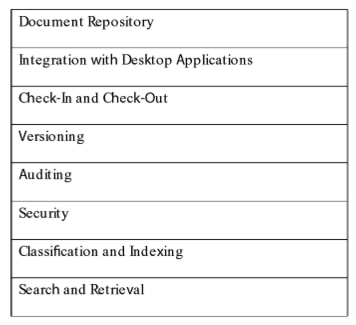
\includegraphics[scale=0.7]{res/bg-knowledge/edms-components.png}
	\caption{Basic components of EDMS \cite{1_adam_2008}}
	\label{fig:edms-components}
\end{wrapfigure}
Later on in the 1990s, Electronics Document Management System (EDMS) is developed targeting large enterprises with high volume of documents.
It is the improved version of DIP with workflow functionality.
Workflow functionality enables organizations to passed around scanned document throughout the organization to designated employee.
EDMS also has its own document repository allowing documents to be indexed and tracked using version control.
There are various sub-types of EDMS such as Electronic Record Management Systems (ERMS) deals mainly with record keeping.
Enterprise Content Management (ECM), suites of applications, deals with document and record management.
Nowadays EDMS acronym is shortened to DMS.
Figure \ref{fig:edms-components} shows a basic components of DMS.
Most DMS applications have these components implemented within.
